\subsection{Lexikální analýza}
\label{subsec:lexer}
Úlohou Lexikálního analyzátoru je rozpoznávat jazykové lexémy a reprezentovat
je jako tokeny.

Lexikální analyzátor je implementací deterministického konečného
automatu. Jediný nedeterministický případ nastává tehdy, když má automat načítat znak ve tvatu $\backslash$ddd.
Případ je vyřešen implementací interního čítače počtu číslic. Pokud čítač dosáhne hodnoty 3 a číslo je
v intervalu $<001-255>$, je znak úspěšné načten, v opačném případě je vygenerována chyba

Lexikální analyzátor je rozdělen do tří modulů: \ic|lexer.c|, \ic|lexer_fsm.c| a \ic|token.c|
. Modul \ic|token.c| obsahuje implementaci abstraktního datového typu token. Modul \ic|lexer_fsm.c|
obsahuje implementaci deterministického konečného automatu. Modul \ic|lexer.c| poskytuje funkci
\ic|lexer_next_token|, která řídí činnost deterministického konečného automatu a
která vrací další token.

\vspace*{16px}
\begin{figure}[htbp]
    \centering
    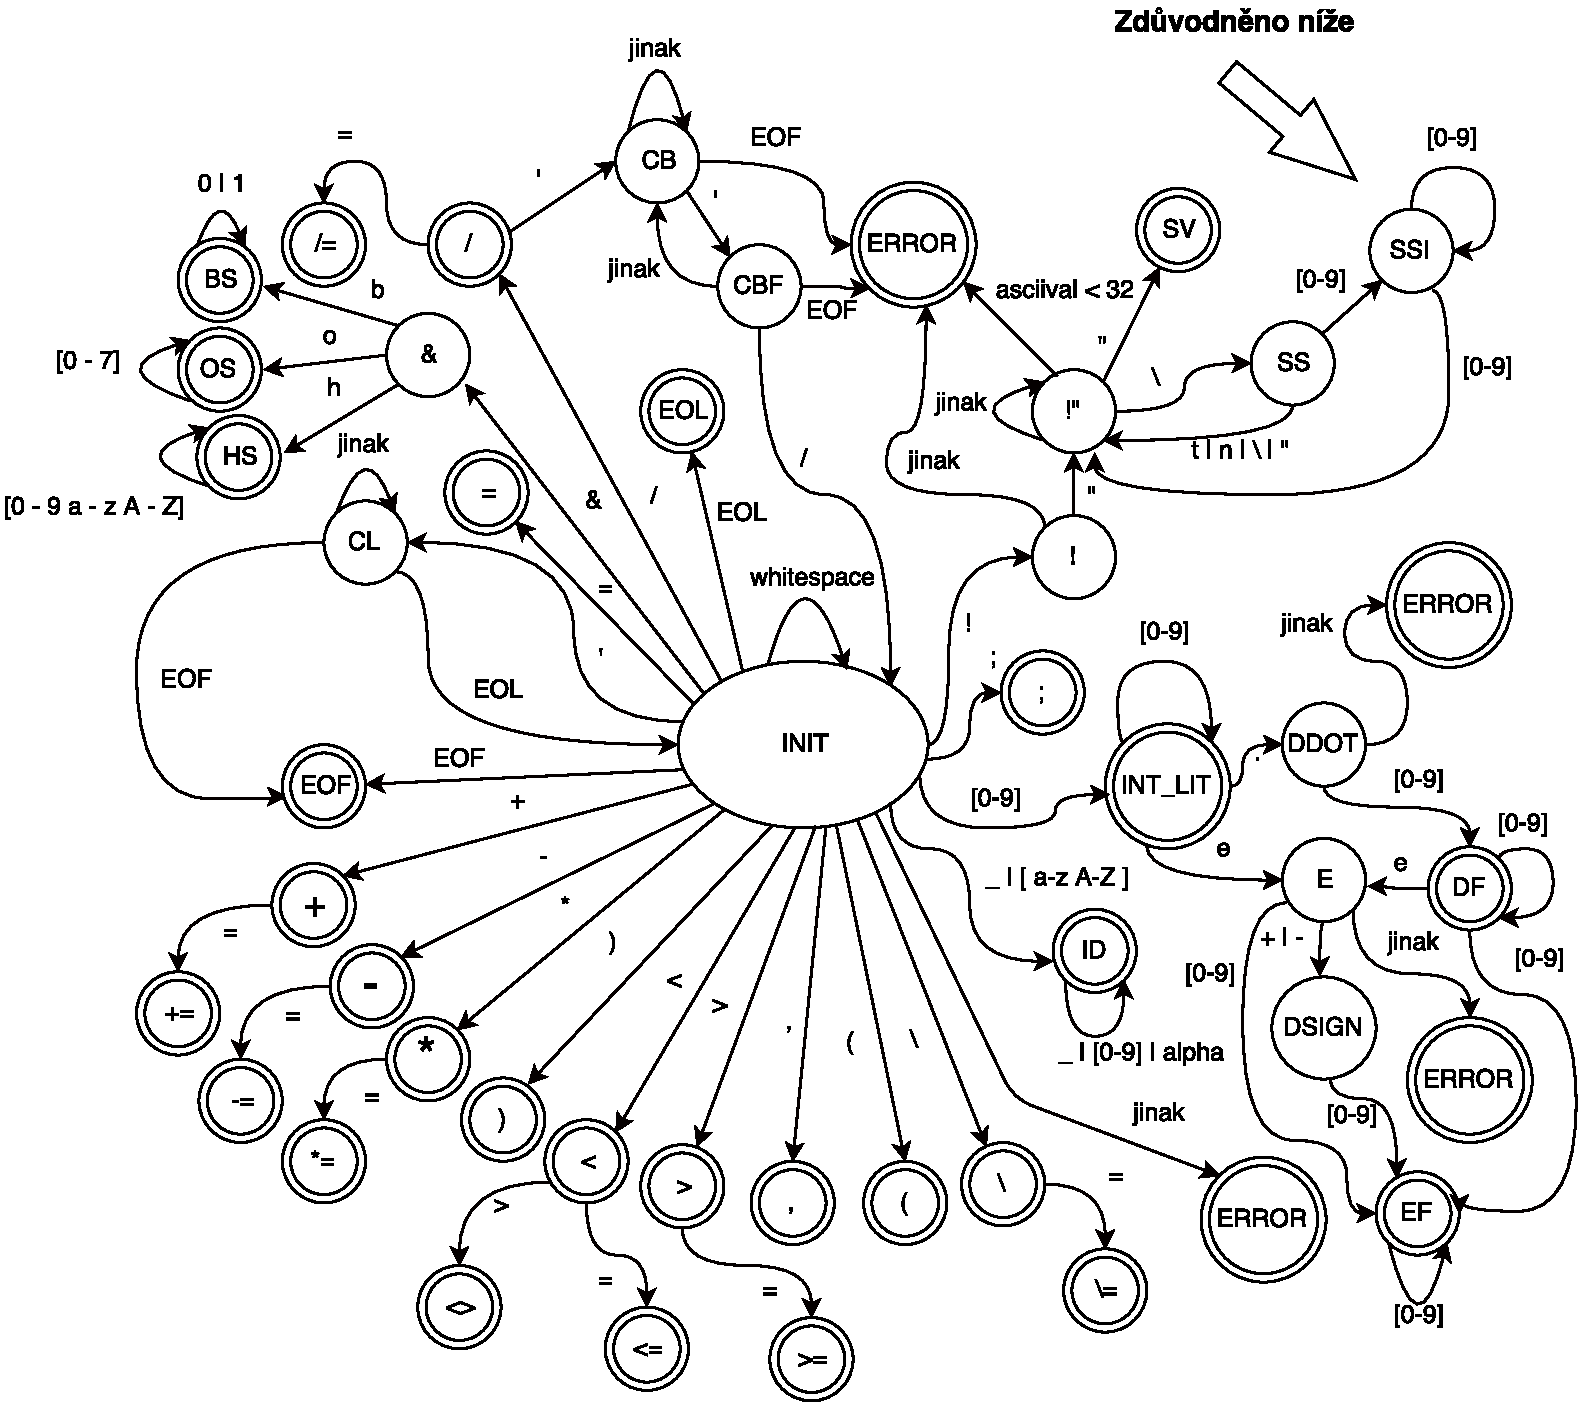
\includegraphics[width=1\textwidth, angle=0]{src/assets/automat.pdf}
\end{figure}

\subsection{Synataktická analýza}
Syntaxí řízený překlad je naimplementován v modulu \ic|parser.c|, pro syntaktickou analýzu programu jako takového je
použita SA shoda dolů, konkrétně metoda rekurzivního sestupu. Pro každé pravidlo z LL gramatiky existuje v tomto
modulu funkce realizující toto pravidlo.

Pro snažší zápis v jazyce C byl implementován poloautomatický systém generování funkcí reprezentujících tato pravidla za pomocí maker.
Makra konkrétní pravidlo zavolají a zkontrolují jeho splnění. Pro kontrolu terminálu bylo naimplemntováno makro
\ic|CHECK_TOKEN(TOKEN_TYPE)|,
Pro zavolání pravidla bylo naimplementováno pravidlo \ic|CALL_RULE(NAME_OF_RULE);|.
Pro podmínečná volání pravidel poté makro ve stylu
\ic|CHECK_RULE(token_type == TOKEN_TYPE, NAME_OF_RULE, REWIND_AND_SUCCESS)| - Pri použití se zavolá pravidlo
\ic|NAME_OF_RULE| v případě, že je následující token typu \ic|TOKEN_TYPE| a jestliže bylo úspěšné, další načtený
token navrátí zpět a prohlásí volání za úspěšné.

Všechny pravidla pracují nad strukturou \ic|Parser|, která zapouzdřuje základní komponenty pro syntaxí řízený překlad.
Jedná se především od struktury \ic!ParserSemantic!, \ic!CodeConstructor! a \ic!Lexer!. První zmíněná zajištuje sémantické
kontroly programu; uchovává \emph{registr symbolů}, dočasné proměnné, pravidla pro implicitní konverze datových typů či
aktuální scénář SA. Konstruktor kódu je poté popsán v příslušné sekci \ref{subsec:code-constructor}, Lexer v sekci
\ref{subsec:lexer}.

Pro analýzu výrazů není analýza shora dolů příliš vhodná, proto byla
použita metoda zdola nahoru v našem případě založená na precedenční
syntaktické analýza implementovaná v souboru \ic|parser_expr.c|.

Přepínání mezi metodami je realizováno následujícím mechanismem. Na celý program je použita funkce \ic|parser_parse|
z modulu \ic|parser.c|. V případě že je jako neterminál očekáván výraz, je volána funkce \ic|parser_parse_expr|
z modulu \ic|parser_expr.c|, která provede precedenční syntaktickou analýzu výrazu.

Pravidlo <statements> obsahuje i derivace, které nemohou v určitém kontextu nastat.
Například return se nemůže vyskytovat v hlavním bloku. Kdybychom toto chtěli řešit
přímo pomocí gramatiky, bylo by to možné ale gramatika by narozstla do monstrózních rozměrů.
Proto nám v tomto napomáhají sémantické akce.

\subsubsection{Gramatika}
\begin{normalsize}
\begin{enumerate}
\item <prog> $\rightarrow$ <body> <eols> EOF
\item <body> $\rightarrow$ <definitions\_block> <scope> <shared\_variables\_declarations>

\item <definitions\_block> $\rightarrow$ <eols> <definitions>

\item <definitions> $\rightarrow$ <definition> <definitions\_block>
\item <definitions> $\rightarrow$ $\varepsilon$

\item <definition> $\rightarrow$ <function\_declaration>
\item <definition> $\rightarrow$ <function\_definition>
\item <definition> $\rightarrow$ <shared\_variable\_declaration>

\item <function\_definition> $\rightarrow$ <function\_header> EOL <eols> <statements> END FUNCTION
\item <function\_declaration> $\rightarrow$ DECLARE <function\_header> EOL <eols>

\item <function\_header> $\rightarrow$ FUNCTION IDENTIFIER (<function\_params>) AS <type>

\item <function\_params> $\rightarrow$ $\varepsilon$
\item <function\_params> $\rightarrow$ <function\_param> <function\_n\_param>

\item <function\_n\_param> $\rightarrow$ $\varepsilon$
\item <function\_n\_param> $\rightarrow$ <function\_param> <function\_n\_param>

\item <function\_param> $\rightarrow$ IDENTIFIER AS <type>


\item <type> $\rightarrow$ INTEGER
\item <type> $\rightarrow$ BOOLEAN
\item <type> $\rightarrow$ STRING
\item <type> $\rightarrow$ DOUBLE

\item <statements> $\rightarrow$ $\varepsilon$
\item <statements> $\rightarrow$ <statement\_single> EOL <eols> <statements>


\item <statement\_single> $\rightarrow$ <identifier\_assignment>
\item <statement\_single> $\rightarrow$ <input>
\item <statement\_single> $\rightarrow$ <return>
\item <statement\_single> $\rightarrow$ <print>
\item <statement\_single> $\rightarrow$ <condition>
\item <statement\_single> $\rightarrow$ <while\_>
\item <statement\_single> $\rightarrow$ <variable\_declaration>
\item <statement\_single> $\rightarrow$ <static\_variable\_declaration>
\item <statement\_single> $\rightarrow$ <scope>

\item <variable\_declaration> $\rightarrow$ DIM IDENTIFIER AS <type> <declaration\_assignment>
\item <declaration\_assignment> $\rightarrow$ E
\item <declaration\_assignment> $\rightarrow$ <assignment>

\item <shared\_variables\_declarations> $\rightarrow$ E
\item <shared\_variables\_declarations> $\rightarrow$ <shared\_variable\_declaration>
\item <shared\_variable\_declaration> $\rightarrow$ DIM SHARED IDENTIFIER AS <type> <declaration\_assignment>

\item <static\_variable\_declaration> $\rightarrow$ STATIC IDENTIFIER AS <type> <declaration\_assignment>

\item <return> $\rightarrow$ RETURN <expr>

\item <assignment> $\rightarrow$ = <expression>
\item <assignment> $\rightarrow$ <modify> <expression>
\item <modify> $\rightarrow$ +=
\item <modify> $\rightarrow$ -=
\item <modify> $\rightarrow$ *=
\item <modify> $\rightarrow$ /=
\item <modify> $\rightarrow$ $\backslash$=

\item <print> $\rightarrow$ PRINT <print\_expression> <print\_expressions>
\item <print\_expressions> $\rightarrow$ E
\item <print\_expressions> $\rightarrow$ <print\_expression> <print\_expressions>
\item <print\_expression> $\rightarrow$ <expression> SEMICOLON

\item <while\_> $\rightarrow$ DO WHILE <expression> EOL <eols> <cycle\_statements> LOOP

\item <input> $\rightarrow$ INPUT IDENTIFIER

\item <identifier\_assignment> $\rightarrow$  IDENTIF <assignment>

\item <condition> $\rightarrow$ IF <expr> THEN EOL <eols> <statements> <condition\_elseif> <condition\_else> END IF
\item <condition\_elseif> <condition\_else>
\item <condition\_elseif> $\rightarrow$ $\varepsilon$
\item <condition\_elseif> $\rightarrow$ ELSEIF <expr> THEN EOL <eols> <statements> <condition\_elseif>

\item <condition\_else> $\rightarrow$ $\varepsilon$
\item <condition\_else> $\rightarrow$ ELSE EOL <eols> <statements>

\item <eols> $\rightarrow$ $\varepsilon$
\item <eols> $\rightarrow$ EOL <eols>

\newpage
\begin{landscape}
\begin{table}[htbp]
\label{table:prec}
\centering
\caption{LL tabulka 1. část}
\begin{tabular}{|l|l|l|l|l|l|l|l|l|l|l|l|l|l|l|l|l|l|l|l|l|l|l|l|l|}
\hline
& {\rotatebox[origin=c]{90}{Operátor}}  & ( & ) & {\rotatebox[origin=c]{90}{identifier}}
& {\rotatebox[origin=c]{90}{integer literal}} & = & ; & {\rotatebox[origin=c]{90}{as}}
& {\rotatebox[origin=c]{90}{asc}}

& {\rotatebox[origin=c]{90}{delcare}} & {\rotatebox[origin=c]{90}{dim}}
& {\rotatebox[origin=c]{90}{do}} & {\rotatebox[origin=c]{90}{double}}
& {\rotatebox[origin=c]{90}{else}} & {\rotatebox[origin=c]{90}{end}}
& {\rotatebox[origin=c]{90}{chr}} & {\rotatebox[origin=c]{90}{function}}

& {\rotatebox[origin=c]{90}{if}} & {\rotatebox[origin=c]{90}{input}}
& {\rotatebox[origin=c]{90}{integer}} & {\rotatebox[origin=c]{90}{length}}
& {\rotatebox[origin=c]{90}{loop}} & {\rotatebox[origin=c]{90}{print}}
& {\rotatebox[origin=c]{90}{return}}
\\ \hline

<prog>&&&&&&&&&&1&&&&&&&1&&&&&&&
\\ \hline
<body>&&&&&&&&&&2&&&&&&&2&&&&&&&
\\ \hline
<def\_b>&&&&&&&&&&3&&&&&&&3&&&&&&&
\\ \hline
<defs>&&&&&&&&&&4&&&&&&&4&&&&&&&
\\ \hline
<def>&&&&&&&&&&6&&&&&&&7&&&&&&&
\\ \hline
<f\_def>&&&&&&&&&&&&&&&&&9&&&&&&&
\\ \hline
<f\_he>&&&&&&&&&&&&&&&&&10&&&&&&&
\\ \hline
<f\_pas>&&&12&13&&&&&&&&&&&&&&&&&&&&
\\ \hline
<f\_n\_p>&&&14&15&&&&&&&&&&&&&&&&&&&&
\\ \hline
<f\_pa>&&&&16&&&&&&&&&&&&&&&&&&&&
\\ \hline
<type>&&&&&&&&&&&&&20&&&&&&&17&&&&
\\ \hline
<sts>&&&&&&&&&&&&&&&21&&&&&&&&&
\\ \hline
<stsi>&&&23&&&&&&&&29&28&&&&&&27&24&&&&26&25
\\ \hline
<va\_de>&&&&&&&&&&&32&&&&&&&&&&&&&
\\ \hline
<va\_as>&&&&&&34&&&&&32&&&&&&&&&&&&&
\\ \hline
<s\_v\_ds>&&&&&&&&&&35&36&&&&&&35&&&&&&&
\\ \hline
<st\_v\_d>&&&&&&&&&&35&36&&&&&&35&&&&&&&
\\ \hline
<ret>&&&&&&&&&&&&&&&&&&&&&&&&39
\\ \hline
<ass>&&&&&&40&&&&&&&&&&&&&&&&&&
\\ \hline
<mod>&&&&&&&&&&&&&&&&&&&&&&&&
\\ \hline
<pr>&&&&&&&&&&&&&&&&&&&&&&&47&
\\ \hline
<pr\_es>&49&49&49&&&&&&&&&&&&&&&&&&&&48&
\\ \hline
<pr\_e>&50&50&50&&&&&&&&&&&&&&&&&&&&&
\\ \hline
<while>&&&&&&&&&&&&51&&&&&&&&&&&&
\\ \hline
<input>&&&&&&&&&&&&&&&&&&&52&&&&&
\\ \hline
<id\_a>&&&&53&&&&&&&&&&&&&&&&&&&&
\\ \hline
<con>&&&&&&&&&&&&&&&&&&54&&&&&&
\\ \hline
<con\_ei>&&&&&&&&&&&&&&&&&&54&&&&&&
\\ \hline
<con\_e>&&&&&&&&&&&&&&&&&&&&&&&&
\\ \hline
<con\_eols>&60&60&60&60&60&60&60&60&60&60&60&60&60&60&60&60&60&60&60&60&60&60&60&60
\\ \hline
\end{tabular}
\end{table}
\end{landscape}
\newpage
\begin{landscape}
\begin{table}[htbp]
    \label{table:prec2}
    \centering
    \caption{LL tabulka 2. část}
\begin{tabular}{|l|l|l|l|l|l|l|l|l|l|l|l|l|l|l|l|l|l|l|l|l|l|l|l|l|l|l|l|l|l|}
\hline


 & {\rotatebox[origin=c]{90}{scope}}
& {\rotatebox[origin=c]{90}{string}} & {\rotatebox[origin=c]{90}{substr}}
& {\rotatebox[origin=c]{90}{then}} & {\rotatebox[origin=c]{90}{while}}
& {\rotatebox[origin=c]{90}{and}} & {\rotatebox[origin=c]{90}{boolean}}
& {\rotatebox[origin=c]{90}{continue}} & {\rotatebox[origin=c]{90}{elseif}}
& {\rotatebox[origin=c]{90}{exit}} & {\rotatebox[origin=c]{90}{false}}
& {\rotatebox[origin=c]{90}{for}} & {\rotatebox[origin=c]{90}{next}}
& {\rotatebox[origin=c]{90}{not}} & {\rotatebox[origin=c]{90}{or}}
& {\rotatebox[origin=c]{90}{shared}} & {\rotatebox[origin=c]{90}{static}}
& {\rotatebox[origin=c]{90}{true}} & {\rotatebox[origin=c]{90}{double literal}}
& {\rotatebox[origin=c]{90}{string value}} & {\rotatebox[origin=c]{90}{comma}}
& {\rotatebox[origin=c]{90}{EOL}}
& {\rotatebox[origin=c]{90}{error}} & {\rotatebox[origin=c]{90}{EOF}}
& {\rotatebox[origin=c]{90}{+=}} & {\rotatebox[origin=c]{90}{-=}}
& {\rotatebox[origin=c]{90}{*=}} & {\rotatebox[origin=c]{90}{/=}}
& {\rotatebox[origin=c]{90}{\textbackslash=}}
\\ \hline
<prog>&1&&&&&&&&&&&&&&&1&&&&&&1&&&&&&&
\\ \hline
<body>&2&&&&&&&&&&&&&&&2&&&&&&2&&&&&&&
\\ \hline
<def\_b>&3&&&&&&&&&&&&&&&3&&&&&&3&&&&&&&
\\ \hline
<defs>&5&&&&&&&&&&&&&&&4&&&&&&&&&&&&&
\\ \hline
<def>&5&&&&&&&&&&&&&&&8&&&&&&&&&&&&&
\\ \hline
<f\_def>&&&&&&&&&&&&&&&&&&&&&&&&&&&&&
\\ \hline
<f\_he>&&&&&&&&&&&&&&&&&&&&&&&&&&&&&
\\ \hline
<f\_pas>&&&&&&&&&&&&&&&&&&&&&&&&&&&&&
\\ \hline
<f\_n\_p>&&&&&&&&&&&&&&&&&&&&&&&&&&&&&
\\ \hline
<f\_pa>&&&&&&&&&&&&&&&&&&&&&&&&&&&&&
\\ \hline
<type>&&19&&&&&18&&&&&&&&&&&&&&&&&&&&&&
\\ \hline
<sts>&&&&&&&&&&&&&&&&&&&&&&&&&&&&&
\\ \hline
<va\_de>&&&&&&&&&&&&&&&&&&&&&&&&&&&&&
\\ \hline
<va\_as>&&&&&&&&&&&&&&&&&&&&&&33&&&&&&&
\\ \hline
<s\_v\_ds>&1&&&&&&&&&&&&&&&&&&&&&&&&&&&&
\\ \hline
<st\_v\_d>&&&&&&&&&&&&&&&&&38&&&&&&&&&&&&
\\ \hline
<ret>&&&&&&&&&&&&&&&&&&&&&&&&&&&&&
\\ \hline
<ass>&&&&&&&&&&&&&&&&&&&&&&&&&41&41&41&41&41
\\ \hline
<mod>&&&&&&&&&&&&&&&&&&&&&&&&&42&43&44&45&46
\\ \hline
<pr>&&&&&&&&&&&&&&&&&&&&&&&&&&&&&
\\ \hline
<pr\_es>&&&49&&&&&&&&&&&&&&&&&&&48&&&&&&&
\\ \hline
<pr\_e>&&&50&&&&&&&&&&&&&&&&&&&&&&&&&&
\\ \hline
<while>&&&&&&&&&&&&&&&&&&&&&&&&&&&&&
\\ \hline
<input>&&&&&&&&&&&&&&&&&&&&&&&&&&&&&
\\ \hline
<id\_a>&&&&&&&&&&&&&&&&&&&&&&&&&&&&&
\\ \hline
<con>&&&&&&&&&&&&&&&&&&&&&&&&&&&&&
\\ \hline
<con\_ei>&&&&&&&&&&&&&&&&&&&&&&&&&&&&&
\\ \hline
<con\_e>&&&&&&&&&&&&&&&&&&&&&&&&&&&&&
\\ \hline
<con\_eols>&60&60&60&60&60&60&60&60&60&60&60&60&60&60&60&60&60&60&60&60&60&61&60&60&60&60&60&60&60

\\ \hline
\end{tabular}

\end{table}
\end{landscape}
\newpage
\end{enumerate}
\end{normalsize}
\subsection{Precedenční analýza výrazů}
Precedenční analýza je řízena precedenční tabulkou, kterou se vyhodnocuje pořadí zpracování tokenů. \ref{table:prec}
\ic|parser_expr_prec_table_data.c|. V tabulce se nachází jak binární, tak i unární mínus. 
Lexikální analyzátor nám ovšem poskytuje pouze jeden token mínus a proto se unární a binární mínus
musí vyhodnotit podle kontextu.

Precedenční analýza využívá zásobníku v podobě obousměrně vázaného seznamu, do kterého se ukládají terminály,
precedenční symboly a neterminály. Pomocí redukčních pravidel, která jsou vypsána v příloze, se postupně výraz redukuje. 
Jelikož překladač je založen na přímém překladu, tak při redukování pomocí pravidel konstruktor kódu rovnou generuje kód programu.

\subsubsection{Redukční pravidla}


\begin{table}[htbp]
\centering
\label{Redukční pravidla}
\begin{tabular}{lll}
    $E \to i$ &  $E \to (E)$ & $E \to (E)$ \\
    $E \to (E)$ & $E \to i()$ & $E \to i(E)$\\
    $E \to i(E, E)$ & $E \to i(E, E, ...)$ &  $E \to E + E$\\
    $E \to E - E$ & $E \to E ~ / ~ E$ & $E \to E ~ \backslash ~ E$\\
    $E \to - E$ &  $E \to E = E$ & $E \to E <> E$\\
    $E \to E > E$ & $E \to E >= E$ & $E \to E < E$\\
    $E \to E <= E$ & $E \to NOT ~ E$ & $E \to E ~ AND ~ E$\\
    $E \to E ~ OR ~ E$ & & \\
\end{tabular}
\end{table}


\begin{table}[htbp]
\label{table:prec}
\centering
\caption{Precedenční tabulka}
\label{precedencni-tabulka}
\begin{tabular}{|l|l|l|l|l|l|l|l|l|l|l|l|l|l|l|l|l|l|l|l|l|}
\hline
 & $un -$ & $*$ & $/$ & $\backslash$ & $+$ & $-$ & $=$ & $<>$ & $<$ & $<=$ & $>=$ & $>$ & $NOT$ & $AND$ & $OR$ & $($ & $)$ & $,$ & $i$ & \$ \\ \hline
$un -$ &$<$&$>$&$>$&$>$&$>$&$>$&$>$&$>$&$>$&$>$&$>$&$>$& x &$>$&$>$&$<$&$>$&$>$&$<$&$>$\\ \hline
$*$ &$<$&$>$&$>$&$>$&$>$&$>$&$>$&$>$&$>$&$>$&$>$&$>$&$<$&$>$&$>$&$<$&$>$&$>$&$<$&$>$\\ \hline
$/$ &$<$&$>$&$>$&$>$&$>$&$>$&$>$&$>$&$>$&$>$&$>$&$>$&$<$&$>$&$>$&$<$&$>$&$>$&$<$&$>$\\ \hline
$\backslash$ &$<$&$<$&$<$&$>$&$>$&$>$&$>$&$>$&$>$&$>$&$>$&$>$&$<$&$>$&$>$&$<$&$>$&$>$&$<$&$>$\\ \hline
$+$ &$<$&$<$&$<$&$<$&$>$&$>$&$>$&$>$&$>$&$>$&$>$&$>$&$<$&$>$&$>$&$<$&$>$&$>$&$<$&$>$\\ \hline
$-$ &$<$&$<$&$<$&$<$&$>$&$>$&$>$&$>$&$>$&$>$&$>$&$>$&$<$&$>$&$>$&$<$&$>$&$>$&$<$&$>$\\ \hline
$=$ &$<$&$<$&$<$&$<$&$<$&$<$& x & x & x & x & x & x &$<$&$>$&$>$&$<$&$>$&$>$&$<$&$>$\\ \hline
$<>$ &$<$&$<$&$<$&$<$&$<$&$<$& x & x & x & x & x & x &$<$&$>$&$>$&$<$&$>$&$>$&$<$&$>$\\ \hline
$<$ &$<$&$<$&$<$&$<$&$<$&$<$& x & x & x & x & x & x &$<$&$>$&$>$&$<$&$>$&$>$&$<$&$>$\\ \hline
$<=$ &$<$&$<$&$<$&$<$&$<$&$<$& x & x & x & x & x & x &$<$&$>$&$>$&$<$&$>$&$>$&$<$&$>$\\ \hline
$>=$ &$<$&$<$&$<$&$<$&$<$&$<$& x & x & x & x & x & x &$<$&$>$&$>$&$<$&$>$&$>$&$<$&$>$\\ \hline
$>$ &$<$&$<$&$<$&$<$&$<$&$<$& x & x & x & x & x & x &$<$&$>$&$>$&$<$&$>$&$>$&$<$&$>$\\ \hline
$NOT$ & x &$>$&$>$&$>$&$>$&$>$&$>$&$>$&$>$&$>$&$>$&$>$&$<$&$>$&$>$&$<$&$>$&$>$&$<$&$>$\\ \hline
$AND$ &$<$&$<$&$<$&$<$&$<$&$<$&$<$&$<$&$<$&$<$&$<$&$<$&$<$&$>$&$>$&$<$&$>$&$>$&$<$&$>$\\ \hline
$OR$ &$<$&$<$&$<$&$<$&$<$&$<$&$<$&$<$&$<$&$<$&$<$&$<$&$<$&$<$&$>$&$<$&$>$&$>$&$<$&$>$\\ \hline
$($ &$<$&$<$&$<$&$<$&$<$&$<$&$<$&$<$&$<$&$<$&$<$&$<$&$<$&$<$&$<$&$<$& = & = &$<$& x \\ \hline
$)$ &$>$&$>$&$>$&$>$&$>$&$>$&$>$&$>$&$>$&$>$&$>$&$>$&$>$&$>$&$>$& x &$>$&$>$& x &$>$\\ \hline
$,$ &$<$&$<$&$<$&$<$&$<$&$<$&$<$&$<$&$<$&$<$&$<$&$<$&$<$&$<$&$<$&$<$& = & = &$<$& x \\ \hline
$i$ & x &$>$&$>$&$>$&$>$&$>$&$>$&$>$&$>$&$>$&$>$&$>$& x &$>$&$>$& = &$>$&$>$& x &$>$\\ \hline
\$ &$<$&$<$&$<$&$<$&$<$&$<$&$<$&$<$&$<$&$<$&$<$&$<$&$<$&$<$&$<$&$<$& x & x &$<$& x\\ \hline
\end{tabular}
\end{table}


\subsection{Sémantická analýza}
Sémantické kontroly jsou přidruženy k syntaktickým pravidlům v rekurzivním sestupu a
precedenční syntaktické analýze výrazů. Jsou organizovány do tzv. scénářů. Jeden
sémantický scénář sémanticky popisuje související část kódu. Například definici
nebo deklaraci funkce. Sémantická analýza nám také pomáhá hlídat některé gramatické aspekty,
které by byly pro LL gramatiku příliš kompikované, nebo by měly příliš dlouhý zápis.


\subsection{Konstruktor kódu}
\label{subsec:code-constructor}
Konstruktor cílového kódu je komponenta překladače, který hlídá význam a odpovědnosti vygenerovaného tříadresného kódu.

\subsection{Generátor cílového kódu}
Generátor kódu je nízkoúrovňová komponenta zastřešující skládání, validaci a vykreslování cílového kódu \ic|IFJcode17|.
Kontroluje generované instrukce a její operandy, tedy správné kombinace typů operandů (přístupy do rámců, konstatní
literály, návěští či datové typy) u konkrétních instrukcí.

Interní implementace spoléhá na \emph{obousměrně svázaný lineární seznam} struktur \ic|CodeInstruction|, které kromě
režijních ukazatelů uchovávají typ instrukce a ukazatele na až tři operandy, struktury \ic|CodeInstructionOperand|.
Tento seznam je uložen v datové struktuře \ic|CodeGenerator|, která dále obsahuje pole podpisů\footnote{Podpis
instrukce je složena z bitových masek definující povolené typy operandů a její textové reprezentace v kódu
\texttt{IFJcode17}.} instrukcí pro jejich validace.
Struktura \ic|CodeInstructionOperand| uchovává informace o svém typu a poté unii dat pro konkrétní typ operandu, tedy
ukazatel na proměnnou \ic|SymbolVariable|,
data konstanty \ic|CodeInstructionOperandConstantData| v unii s datovým typem nebo řetězec uchovávající název návěští.
\subsection{Optimalizátor kódu}
\todo{Sony alespoň pár odstavečků by to chtělo}

\section{Rozšíření}

\subsubsection{SCOPE}
Pro rozšíření bylo třeba upravit tabulku symbolů, sekci proměnných tak, aby
měla zásobníkovou strukturu a umožňovala libovolné operace push a pop na úrovni tabulek.
Dále byly vytvořeny sémantické akce pro vyhledání v libovolné z těchto tabulek,
nebo jen v tabulce která je na vrcholu zásobníku. Definice proměnných v těle cyklu
bylo vyřešeno přesunutím instrukce defvar před cyklus samotný.
\subsubsection{GLOBAL}
Rozšíření GLOBAL bylo zapotřebí implementovat gramaticky přidáním
nových pravidel pro definici statických a globálních proměnných.
Dále bla upravena tabulka proměnných, ve které je jedna tabulka vyhrazena
pro globální proměnné a statické proměnné které jsou prefixovány
jménem funkce ve které se vyskytují.
\subsubsection{UNARY}
Rozšíření UNARY jsme implementovali jako nová gramatická pravidla. Sémantické
akce odpovídají přiřazení, liší se pouze vygenerovaný kód.
\subsubsection{BASE}
Rozšíření bylo implementováno v lexikálním analýzatoru. Jsme schopni rozpoznat
lexémy označující čísla ve dvojkové, osmičkové a šestnáctkové soustavě a
výsledek převést na desítkové číslo se kterým již nakládáme stejně.
\subsubsection{FUNEXP}
Volání funkcí bylo implementováno na úrovni precedenční syntaktické analýzy,
takže lze ve výrazu volat libovolné funkce.
\subsubsection{IFTHEN}
Implementováno na gramatické úrovni přidáním nepovinných částí
elseif a odstraněních povinnosti mít část if.
\subsubsection{BOOLOP}
Bylo potřeba upravit precedenční tabulku tak, aby podporovala nové
operace AND a OR, dále gramatiku tak, abychom jako datový typ mohli
použít typ boolean a sémantické akce pro ověření nového datového typu.